\section{Calibrating the diagnostic}
\label{sec:calib}

The sea-ice benchmark cannot establish sensitivity, because the crop-dependence of
that pipeline is the unknown being estimated. So we built a labeller with a dial. Sen1Floods11~\cite{bonafilia2020sen1floods11}
ships an Otsu-on-VH~\cite{otsu1979threshold} label set with one published threshold
per flood event, whose preprocessing we recover in \Cref{sec:recovery}. Holding that
smoothing fixed and recomputing only the threshold inside each crop reproduces the
sea-ice mechanism with one scalar per crop as the entire source of crop-dependence:
\begin{equation}
\tau_c(\alpha) = (1-\alpha)\,\tau_{\text{event}} + \alpha\,\tau_{\text{crop}} .
\label{eq:dial}
\end{equation}
At $\alpha = 0$ the labels are the published ones, crop-invariant by construction. At
$\alpha = 1$, Otsu returns a crop threshold at 72{,}029 of 75{,}374 positions
(95.56\%); 2{,}331 (3.09\%) use a finite chip fallback, while 1{,}014 positions in
six chips (1.35\%) remain unusable and those chips are excluded from every arm. The within-chip range averages
6.13\,dB. The endpoint also shifts the mean threshold from $-21.798$ to
$-17.796$\,dB. The dial controls crop fitting but does not isolate
crop-dependence.

The artefact set \emph{and the labels it is scored against} are both fixed at
$\alpha = 1$: write $\kap_{L^\star\!,\A^\star}(f_\alpha)$ for the model trained at
$\alpha$ read against that fixed reference. Rebuilding either per arm would empty
$\A$ at $\alpha = 0$, leaving the control with no pixels to be null on. So $\kap$
there is an empirical near-zero from a model that never learned the artefact; it is
separate from the proposition's identity. Sea ice works the same way.

\begin{figure}[tb]
\centering
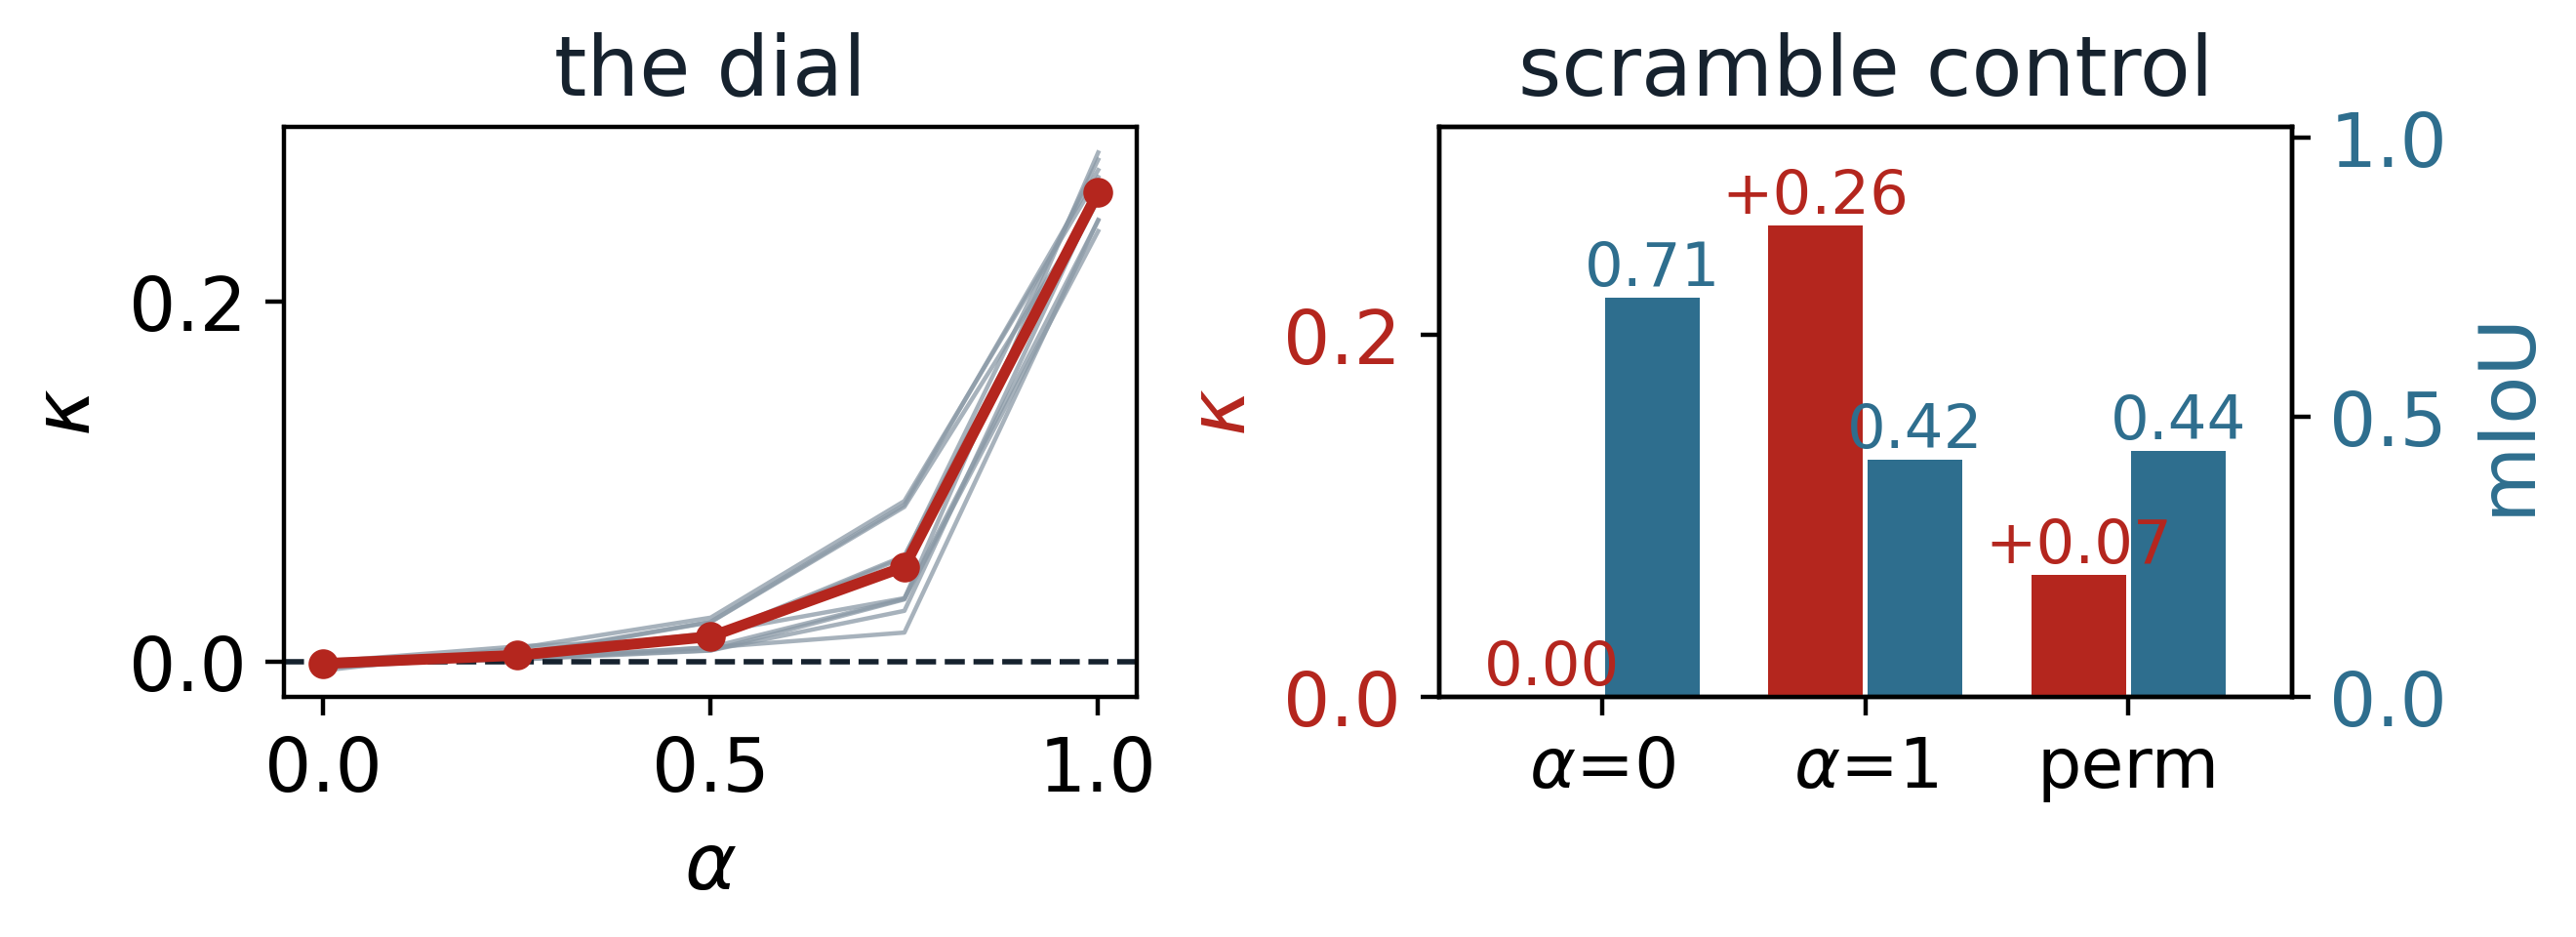
\includegraphics[width=\linewidth]{figures/fig4_calibration.png}
\caption{Left: $\kap$ against the dial of \cref{eq:dial}, grey lines held-out events
and red the mean; the dashed line marks the algebraic zero. $\alpha = 0$ is the
published threshold, while $\alpha = 1$ is
predominantly crop-fitted (95.56\% direct fits; the remainder is accounted for in text).
Right: those arms and \emph{scramble}, one random reassignment of threshold positions
within each chip; $\kap$ red on the left axis, mIoU against expert labels blue on the
right. It preserves the threshold multiset but does not eliminate spatial dependence.}
\label{fig:calib}
\end{figure}

\begin{table}[tb]
\centering
\scriptsize
\setlength{\tabcolsep}{1.3pt}
\resizebox{\linewidth}{!}{%
\begin{tabular}{@{}lccccc|cc@{}}
\toprule
 & \multicolumn{5}{c|}{dial, $\alpha$} & \multicolumn{2}{c}{controls} \\
 & 0.00 & 0.25 & 0.50 & 0.75 & 1.00 & scramble & offset \\
\midrule
$\kap$   & $-0.0008$ & $+0.0037$ & $+0.0141$ & $+0.0528$ & $\mathbf{+0.2605}$ & $+0.0672$ & $-0.0003$ \\
$\Omega$ & 0.0108 & 0.0132 & 0.0211 & 0.0454 & 0.1119 & 0.0933 & 0.0121 \\
mIoU     & 0.714 & 0.696 & 0.673 & 0.604 & $\mathbf{0.423}$ & 0.440 & 0.715 \\
\bottomrule
\end{tabular}
}
\caption{Crop-label alignment, model crop-dependence and accuracy against expert
labels, averaged descriptively over the eleven held-out events. Every $\kap$ uses the
same $\alpha=1$ reference set, with $P(\A^\star)=24.71\%$. \emph{Scramble} randomly
reassigns thresholds within each chip; \emph{offset} is constant within a chip and
varies only between chips.}
\label{tab:calib}
\end{table}

The three diagnostics in \cref{tab:calib} answer different questions. The fixed
$P(\A^\star)$ is a label-only prevalence and cannot rank these models; $\Omega$ is
unsigned prediction inconsistency and remains positive for both near-zero controls.
Only $\kap$ records the signed association between a prediction and the label of the
particular crop being read.

\cref{tab:calib} and \cref{fig:calib} give the result. The contrast between the ends
is $+0.2613$ (sd $0.0149$), positive in 11 of 11 events after averaging seeds within
event, and per-event rank
correlation with $\alpha$ is perfect in all eleven. At
$\alpha = 0$, where the labels are the published ones and crop-invariant exactly,
$\kap$ reads $-0.0008$.

\paragraph{What changes across the dial.} A threshold recomputed on a water-poor
$128 \times 128$ window is not only crop-dependent, it is worse: accuracy against
expert labels falls by $0.29$ mIoU across the dial. None of the dial values isolates
crop adaptation from the accompanying changes in threshold and label quality. The
scramble arm is a sensitivity check and does not isolate causality. Within
each chip it preserves the exact threshold multiset, but the unconstrained random
permutation leaves 461 of 75{,}374 assignments (0.61\%) fixed and pairs 21.78\% of
recipients with a geometrically overlapping donor crop; all donors also share the
same chip. These geometry counts describe the full serialized mapping, including
the six chip rows excluded from training and scoring. In this one reassignment, model performance retained 94\% of the endpoint
mIoU difference ($-0.2736$ versus $-0.2905$), while $\kap$ fell from $+0.2605$ to
$+0.0672$, leaving 26\% of the endpoint excess. That residual cannot be partitioned
among generic crop-varying labels, overlap, and same-chip predictability. The offset
arm, varying the threshold once per chip at the same spread, yields $-0.0003$.

\paragraph{Dependence of fold summaries.} The eleven events are distinct, but
the eleven models are leave-one-event-out folds sharing nearly all of their
training data, so a $t$ or a sign test over them assumes an independence the
design does not provide, exactly as on sea ice. \Cref{tab:seeds} offers
a training-seed sensitivity check instead: the aggregate contrasts vary by less
than $0.011$ across three seeds. This shows stability on the same folds. It does not
provide independent replication or reassignment uncertainty because all three seeds
use the same scramble; Table~\ref{tab:seeds} lists those seed-wise contrasts.

\begin{table}[tb]
\centering
\footnotesize
\setlength{\tabcolsep}{4pt}
\begin{tabular}{lccc}
\toprule
contrast & seed 7 & seed 42 & seed 123 \\
\midrule
$\alpha{=}1$ against $\alpha{=}0$ & $+0.2601$ & $+0.2666$ & $+0.2573$ \\
$\alpha{=}1$ against scramble & $+0.1992$ & $+0.1919$ & $+0.1888$ \\
\bottomrule
\end{tabular}
\caption{Training-seed sensitivity of the dial. Each cell is the mean over the same
eleven held-out events, so the exact ranges across seeds are $0.0093$ and $0.0104$ against
effects of $+0.26$ and $+0.19$.}
\label{tab:seeds}
\end{table}

\paragraph{Scope.} Sen1Floods11 as published computes one threshold per event, so the
crop-dependent artefact is not present in that benchmark. The imagery and the labeller
are real and the crop-dependence is ours. This experiment calibrates the diagnostic;
it does not establish a second real-world occurrence, and nothing here bears on that
dataset's published labels.
